%
% -- Настройки класса документа -------------------------------------------

\documentclass[12pt, a4paper, oneside, final]{book} % Класс документа
\usepackage{cmap} 								    % Поиск и копирование текста
\usepackage[T2A]{fontenc} 							% Специалньые символы
\usepackage[utf8]{inputenc} 						% Кодировка
\usepackage[english, russian]{babel} 				% Используемые языки

% -- Настройка шрифтов ----------------------------------------------------

\usepackage[scaled = 0.96, sups]{XCharter} 			 % Bitstream Charter ("< \ "> -- кавычки)
\usepackage[scaled = 1.04, varqu, varl]{inconsolata} 
\usepackage[type1]{cabin} 							 % Шрифт для текста
\usepackage[vvarbb, scaled = 1.12]{newtxmath} 		 % Шрифт для формул (libertine)
\usepackage[cal = boondoxo]{mathalfa} 				 % Гарнитура шрифта для формул
 
% -- Загрузка библиотек ---------------------------------------------------

%\usepackage{amssymb}
\usepackage{amsmath, amsfonts, latexsym} 				% Математическая символика
\usepackage{geometry} 					 				% Поля
\usepackage{setspace}                    				% Коррекция интервалов
\usepackage{indentfirst}                 				% Начало главы с красной строки
% \usepackage[none]{hyphenat}            				% Отключение переноса слов
\usepackage{graphicx}                    				% Графика
\usepackage{titlesec}                    				% Редактирование section и chapter
\usepackage{fancyhdr, fancybox}          				% Редактирование колонтитулов
\usepackage{listings}                    				% Оформление листинга кода с подсветкой
\usepackage{color}                       				% Цвета
\usepackage{hyperref}                    				% Гиперссылки в PDF
\usepackage{nicefrac}                    				% Симпатичные дроби
\usepackage{float}                       				% Настройка плавающего окружения
\usepackage{rotating}                    				% Поворот плавающего окружения
\usepackage{ulem}                        				% Настраиваемое подчеркивание текста
\usepackage{titlesec}                    				% Настройка отображения заголовков
\usepackage{enumitem}                    				% Настройка форматирования нумерованных списков
\usepackage{algorithm}                   				% Использование псевдокодов
\usepackage{algpseudocode}                              % Поддержка русского языка в псевдокодах
\usepackage{tikz}                        				% Создание векторной графики
\usepackage{xfp}                         			    % Поддержка вычислений в коде
\usepackage{framed}                     			    % Выделение блоком текста
\usepackage{pgfplots}                    				% Построение графиков
\usepackage{stanli}                      				% Пакет Tikz для отрисовки конструкций
\usepackage{tabularray}                  				% Таблицы с гибким форматированием
\usepackage{cite}										% Группировка источников при цитировании
\usepackage[labelfont = {it}, textfont = {it}]{caption} % Настройка подписей
\usepackage[nottoc, notlof, notlot]{tocbibind} 			% Отображение списка источников в оглавлении
\graphicspath{{images//}} 								% Путь для картинок (//==рекурсивный поиск директорий)

% -- Опции форматирования ---------------------------------------------------	

\geometry{left = 3cm, right = 1.5cm, top = 2cm, bottom = 2cm} % Настройки полей
\frenchspacing 												  % Одинаковые пробелы
\renewcommand{\baselinestretch}{1.3}					      % Межстрочный интервал
\parindent = 1.25cm 										  % Отступ абзацный
\hyphenpenalty = 5000 										  % Пороговое значение штрафа для переноса слова
% \hbadness = 10000 										  % Отключение предупреждения о проблемных блоках (при hypehenat==on)
\sloppy 													  % Контроль переполнения блоков

% -- Работа с таблицами -----------------------------------------------------

% Tabular и Longtable
\DeclareCaptionLabelFormat{gost-table}{\hfill #1~#2}    % Указатель
\DeclareCaptionTextFormat{gost-table}{\centering #1 \\} % Текст
\captionsetup[table]{textformat = gost-table, labelformat = gost-table, singlelinecheck = off, labelsep = newline} % Задание формата

% Tabularrray
	% Стиль
\NewTblrTheme{regularTable}{
	\SetTblrStyle{caption-tag}{font=\itshape}
	\SetTblrStyle{caption-text}{font=\itshape}
}
\UseTblrLibrary{varwidth}
	% Настройки заголовка первого блока таблиц
\DefTblrTemplate{caption-sep}{default}{}
\DefTblrTemplate{caption}{default}{
\par\hfill
	\UseTblrTemplate{caption-tag}{default}
	\UseTblrTemplate{caption-sep}{default}
	\newline\centering
    \UseTblrTemplate{caption-text}{default}	
   	\par
}
	% Настройки перенесенного заголовка
\DefTblrTemplate{contfoot-text}{default}{}
\DefTblrTemplate{conthead-text}{default}{(продолжение)}
\DefTblrTemplate{capcont}{default}{
\par\hfill
	\UseTblrTemplate{caption-tag}{default}
	\UseTblrTemplate{caption-sep}{default}
	\newline\centering
    \UseTblrTemplate{caption-text}{default}	
    \UseTblrTemplate{conthead-text}{default}
\par
}

% -- Нумерация страниц ------------------------------------------------------

% Смена заголовков глав и секций
\pagestyle{fancy} % Выбор системного стиля
\renewcommand{\chaptermark}[1]{\markboth{\itshape\thechapter.\ #1}{}} % Главы
\renewcommand{\sectionmark}[1]{\markright{\itshape\thesection.\ #1}}  % Секции

% Базовый стиль (начало глав)
\fancypagestyle{plain}{
	\fancyhf{} 						   % Очистка всех хедеров и футеров
	\fancyfoot[C]{-- \thepage\ --} 	   % Нумерация страницы
	\renewcommand{\headrulewidth}{0pt} % Толщина разделительной полосы сверху
	\renewcommand{\footrulewidth}{0pt} % Толщина разделительной полосы снизу
}
 % Основной стиль
\fancypagestyle{main}{
	\fancyhf{}											   % Очистка всех хедеров и футеров
	% Положение глав
	\fancyhead[L]{\ifodd\value{page} \leftmark \fi} 	   % Нечетные страницы
	\fancyhead[R]{\ifodd\value{page} \else \rightmark \fi} % Четные страницы
	\fancyfoot[C]{-- \thepage\ --} 						   % Нумерация страницы
	\renewcommand{\headrulewidth}{0.2pt} 				   % Толщина разделительной полосы сверху
	\renewcommand{\footrulewidth}{0pt} 					   % Толщина разделительной полосы снизу
}

% Задание дополнительных стилей
	% Стиль нумерации без хедера
\fancypagestyle{onlyNum}{ 
	\fancyhf{} 						   % Очистка всех хедеров и футеров
	\fancyfoot[C]{-- \thepage\ --}     % Нумерация страницы
	\renewcommand{\headrulewidth}{0pt} % Толщина разделительной полосы сверху
	\renewcommand{\footrulewidth}{0pt} % Толщина разделительной полосы снизу
}
	% Стиль нумерации без глав
\fancypagestyle{onlyRightMark}{ 
	\fancyhf{} 														% Очистка всех хедеров и футеров
	\fancyfoot[C]{-- \thepage\ --} 								    % Нумерация страницы
	\fancyhead[R]{\ifodd\value{page} \else \bfseries\rightmark \fi} % Четные страницы
	\fancyfoot[C]{\thepage} 										% Нумерация страницы
}

%  -- Рубрикация -------------------------------------------------------------

\makeatletter % Используем символ @ как букву
% Запрет переносов в названиях секций
\renewcommand{\section}{\@startsection{section}{1}{0pt}{1ex}{1ex}{\centering\hyphenpenalty=10000\normalfont\bfseries}}

% Смена заголовка для команды \chapter и запрет переноса слов
\titleformat{\chapter}{\centering\hyphenpenalty=10000\normalfont\large\bfseries}{\thechapter. }{0pt}{\large}
\renewcommand\@biblabel[1]{#1.} % Точка перед источниками литературы
\makeatother
\titlespacing*{\chapter}{0pt}{-50pt}{10pt} % Вертикальные отступы от названия главы
\titleformat*{\subsection}{\normalfont\bfseries} % Подраздел

% Кириллический алфавит
\makeatletter
\renewcommand*{\@alph}[1]{% 
  \ifcase#1\or а\or б\or в\or г\or
    д\or е\or ё\or ж\or з\or и\or й\or
    к\or л\or м\or н\or о\or п\or р\or с\or т\or
    у\or ф\or х\or ц\or ч\or
    ш\or щ\or ъ\else\@ctrerr\fi
}
\renewcommand*{\@Alph}[1]{% 
  \ifcase#1\or А\or Б\or В\or Г\or
    Д\or E\or Ё\or Ж\or З\or И\or Й\or
    К\or Л\or М\or Н\or О\or П\or Р\or С\or Т\or
    У\or Ф\or Х\or Ц\or Ч\or
    Ш\or Щ\or Ъ\else\@ctrerr\fi
}
\makeatother

%  -- Листинг кода -------------------------------------------------------------

% Смена названия блока псевдокода
\makeatletter
\renewcommand*{\ALG@name}{Алгоритм}
\makeatother

% Определение именнованных цветов
\definecolor{mygreen}{RGB}{28, 172, 0} 
\definecolor{mylilas}{RGB}{170, 55, 241} 
	
%  Общие настройки
\lstset{
	basicstyle = \small\normalfont,    % Размер и начертание шрифта для подсветки кода
	numbers = left,                    % Где поставить нумерацию строк (слева\справа)
	numberstyle = \tiny,               % Размер шрифта для номеров строк
	stepnumber = 1,                    % Размер шага между двумя номерами строк
	numbersep = 5pt,                   % Как далеко отстоят номера строк от подсвечиваемого кода
	% backgroundcolor = \color{white}, % Цвет фона подсветки
	showspaces = false,                % Показывать или нет пробелы специальными отступами
	showstringspaces = false,          % Показывать или нет пробелы в строках
	showtabs = false,                  % Показывать или нет табуляцию в строках
	frame = tb,                 	   % Рисовать рамку вокруг кода
	tabsize = 2,                       % Размер табуляции по умолчанию равен 2 пробелам
	captionpos = t,                    % Позиция заголовка вверху [t] или внизу [b] 
	breaklines = true,                 % Автоматически переносить строки (да\нет)
	breakatwhitespace = false,         % Переносить строки только если есть пробел
	texcl = true, 			           % Поддержка русских символов (LaTeX коммент.)
}

% Стили языков
	% Matlab 
\lstdefinestyle{Matlab}{ 
	language = Matlab,                                        % Выбор языка для подсветки
	morekeywords = {matlab2tikz},							  % Подгрузка ключевых слов
	keywordstyle = \color{blue},                              % Подсветка ключевых слов
	morekeywords = [2]{1}, keywordstyle = [2]{\color{black}}, % Стиль ключевых слов
	identifierstyle = \color{black},						  % Фильтрация стиля
	stringstyle = \color{mylilas},						      % Цвет строк
	commentstyle = \color{mygreen},						      % Цвет комментариев
	showstringspaces = false, 							      % Пробельный символ
	numbers = left,									          % Нумерация слева
	numberstyle = {\tiny \color{black}},					  % Шрифт нумерации
	numbersep = 9pt, 									      % Отступ нумерации
	emph = [1]{for,end,break}, emphstyle = [1]\color{red}, 	  % Акцент на словах
}	

	% Tree
\lstdefinestyle{tree}{
	language = Matlab, 
	stringstyle = \color{mylilas},	% Цвет строк
	commentstyle = \color{mygreen},	% Цвет комментариев
	showstringspaces = false, 		% Пробельный символ
	numbers = none,					% Нумерация слева	
    literate =						% Замена символов дерева утилиты tree
    {├}{{\smash{\raisebox{-1ex}{\rule{1pt}{\baselineskip}}}\raisebox{0.5ex}{\rule{1ex}{1pt}}}}1 
    {─}{{\raisebox{0.5ex}{\rule{1.5ex}{1pt}}}}1 
    {└}{{\smash{\raisebox{0.5ex}{\rule{1pt}{\dimexpr\baselineskip-1.5ex}}}\raisebox{0.5ex}{\rule{1ex}{1pt}}}}1,
    emph = [1]{Signals, Results, LICENSE, Geometry, Distortion field, Export_fig},emphstyle=[1]\color{red}, 	  % Акцент на словах
}

	% Fortran
\lstdefinestyle{Fortran}{ 
	language = Fortran,                                       % Выбор языка для подсветки
	breaklines = true,									      % Пропуск линий
	keywordstyle = \color{blue},                              % Подсветка ключевых слов
	morekeywords = [2]{1}, keywordstyle = [2]{\color{black}}, % Стиль ключевых слов
	identifierstyle = \color{black},						  % Фильтрация стиля
	stringstyle = \color{mylilas},						      % Цвет строк
	commentstyle = \color{mygreen},						      % Цвет комментариев
	showstringspaces = false, 							      % Пробельный символ
	numbers = left,									          % Нумерация слева
	numberstyle = {\tiny \color{black}},					  % Шрифт нумерации
	numbersep= 9pt, 									      % Отступ нумерации
	emph = [1]{for, end, break}, emphstyle = [1]\color{red},  % Акцент на словах
}	

% -- Работа с графикой --------------------------------------------------------

\usetikzlibrary{shadows, arrows}          % Использование теней и стрелок
\usetikzlibrary{positioning}              % Позиционирование
\usetikzlibrary{patterns}                 % Паттерны заливки
\usetikzlibrary{decorations.pathmorphing} % Декорации
\usetikzlibrary{calc}                     % Расчетная библиотека
\pgfplotsset{compat = newest}             % Версия библиотеки для отрисовки графиков
\usetikzlibrary{trees}   				  % Деревья

% Чертежные виды
\tikzstyle{isometric} = [x = {(0.710cm, -0.410cm)}, y = {(0cm, 0.820cm)}, z = {(-0.710cm,-0.410cm)}]
\tikzstyle{dimetric}  = [x = {(0.935cm, -0.118cm)}, y = {(0cm, 0.943cm)}, z = {(-0.354cm, -0.312cm)}]
\tikzstyle{dimetric2} = [x = {(0.935cm, -0.118cm)}, z = {(0cm, 0.943cm)}, y = {(+0.354cm, +0.312cm)}]
\tikzstyle{trimetric} = [x = {(0.926cm, -0.207cm)},y = {(0cm, 0.837cm)}, z = {(-0.378cm, -0.507cm)}]

% Стили
	% Оси и размеры
\tikzstyle{dim<->} = [thick, latex-latex]              % Двусторонний размер
\tikzstyle{dim->} = [-latex] 						   % Односторонний размер
\tikzstyle{axis} = [thick, -latex', color = black]     % Линия оси координат
\tikzstyle{symLine} = [thick, dash dot, color = black] % Линия симметрии
	% Штриховка
\tikzstyle{hatching1} = [pattern = north east lines]   % Нельзя переопределять hatching из stanli (!)
	% Вектора
\tikzstyle{vector} = [very thick, -latex]

%  -- Дополнительные математические операторы ---------------------------------

\DeclareMathOperator*{\argmax}{arg\,max}
\DeclareMathOperator*{\argmin}{arg\,min}

%  -- Навигация ---------------------------------------------------------------

% Гиперссылки
\hypersetup{ 
    colorlinks = true, 	 % Включить цветные ссылки (print == false)
    linkcolor = blue,	 % Цвет ссылки на объект
    filecolor = magenta, % Цвет ссылки на файл    
    urlcolor = cyan,	 % Цвет ссылки на сайт
    citecolor = green 	 % Цвет ссылки на цитату
}

% -- Завершение статической части преамбулы ------------------------------------

\csname endofdump \endcsname

% ------------------------------------------------------------------------------
%\begin{document}
%
% -- Переименование рубрикации -------------------------------------------------

\renewcommand{\contentsname}{Содержание} 				  % Оглавление -> Содержание
\renewcommand{\bibname}{Список использованных источников} % Литература -> Список использованных источников

% -- Главы и секции без нумерации ---------------------------------------------

\newcommand{\AddNoTocChap}[2]{ % Использование глав без нумерации
\def\temp{#2}\ifx\temp\empty % Проверка типа главы
	\chapter*{#1}  % Введение, заключение...
  	\addcontentsline{toc}{chapter}{#1} \fancyhead{} % Сброс заголовка хедера
\else
  	\chapter*{#1 \\ #2}  % Приложение
  	\addcontentsline{toc}{chapter}{#1. #2} \fancyhead{} % Сброс заголовка хедера
\fi
\fancyhead[L]{\ifodd\value{page} \bfseries \MakeUppercase{#1} \fi} % Нечетные страницы
\fancyhead[R]{\ifodd\value{page} \else \bfseries \MakeUppercase{#1} \fi} % Четные страницы
}

% -- Создание математических формул -------------------------------------------

% Частная производная n-го порядка по одному аргументу
\newcommand{\partDer}[3]{ 
\ifthenelse{ \equal{#3}{1} \OR \equal{#3}{} }
	{ \frac{\partial #1}{\partial #2} }
	{ \frac{\partial^{#3} #1}{\partial #2^{#3}} }
}
% Верхнее подчеркивание
\newcommand{\ol}[1]{ 
 	\overline{#1}
}
\setlength{\abovedisplayskip}{1ex} % Вертикальный отступ перед формульным окружением
\setlength{\belowdisplayskip}{1ex} % Вертикальный отступ после формульного окружения

% -- Сокращения ---------------------------------------------------------------

% Формулы
\newcommand{\nfrac}{\nicefrac}        % Однострочная дробь
\newcommand{\rarr}{$\rightarrow$ }    % Стрелка вправо
\newcommand{\matr}[1]{\mathbf{#1}}    % Жирные матричные символы
\newcommand{\vphi}{\varphi}        	  % Phi
\newcommand{\R}{\mathbb{R}}           % Множество
\newcommand{\imag}{\operatorname{Im}} % Мнимая часть числа
\newcommand{\real}{\operatorname{Re}} % Действительная часть числа

% Рисунки
\newcommand{\figrefb}[1]{рис.~\ref{#1}} % Без скобок
\newcommand{\figref}[1]{(\figrefb{#1})} % Со скобками
% Таблицы
\newcommand{\tabrefb}[1]{табл.~\ref{#1}} % Без скобок
\newcommand{\tabref}[1]{(\tabrefb{#1})}  % Со скобками
% Листинги
\newcommand{\listref}[1]{(лист.~\ref{#1}, c.~\pageref{#1})} 

% -- Обновление fancy ---------------------------------------------------------

\newcommand{\updateFancy}{ 
	\pagestyle{main}
}

% -- Установки по умолчанию ---------------------------------------------------

\updateFancy % Стиль нумерации

% -----------------------------------------------------------------------------
% -- Debug ------------------------------------------------------------------

\chapter{Описание программных возможностей}

С целью обеспечения возможности эффективного расчета обобщенных характеристик по результатам модальных испытаний, была разработана программная реализация «GenCalc», позволяющая посредством графического интерфейса \figref{interface} гибко менять параметры расчета и исследовать зависимости получаемых характеристик по каждому из способов одновременно. Более того, для оценки качества выделения тона
колебаний в программе заложена возможность построения частотного годографа \figref{godograph} и параметра монофазности \figref{monophase-parameter} колебательной системы.

Необходимо отметить, что разработанная программная реализация обеспечивает прямое взаимодействие с результатами модальных испытаний, которые были получены с использованием комплекса Simcenter Testlab.

В рамках предлагаемого подхода, для расчетного диапазона необходимо задать минимальный и максимальный уровень амплитуды, число уровней, а также число точек для интерполяции сигнала отклика на каждом уровне.
Кроме того, необходимо выбрать частоту амплитудного и фазового резонанса.

\begin{figure}[!htb]
	\centering
	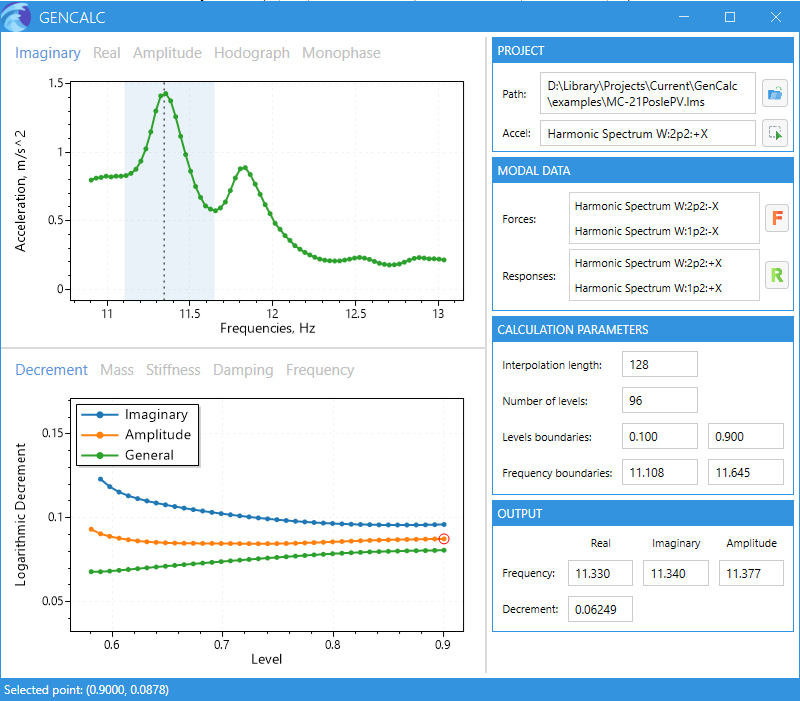
\includegraphics[width=1\linewidth]{interface}
	\caption{Графический интерфейс программы} \label{interface}
\end{figure}

\begin{figure}[H]
	\centering
	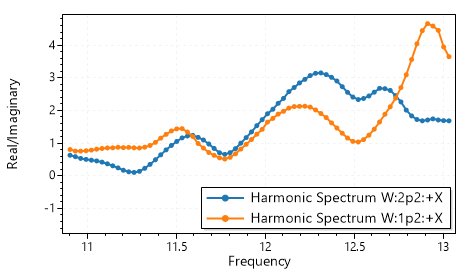
\includegraphics[width=0.8\linewidth]{monophase-parameter}
	\caption{Параметр монофазности по двум каналам возбуждения при колебаниях изделия по тону АГИКр2} \label{monophase-parameter}
\end{figure}

\begin{figure}[!htb]
	\centering
	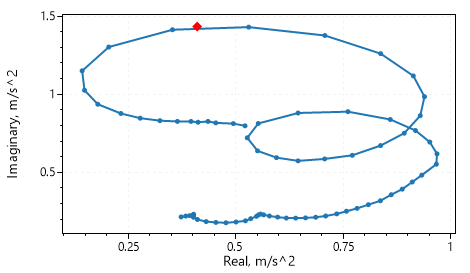
\includegraphics[width=0.8\linewidth]{godograph}
	\caption{Частотный годограф в точке отклика изделия при колебаниях
по тону АГИКр2} \label{godograph}
\end{figure}

\chapter{Описание расчетной методики}

Программный функционал позволяет определять логарифмической декремент колебаний системы по каждому тону, используя четыре подхода:
\begin{enumerate}[topsep=0pt, noitemsep]
	\item По ширине резонансного пика мнимой составляющей сигнала отклика.
	\item По ширине резонансного пика амплитуды колебаний.
	\item По наклону реальной составляющей сигнала отклика.
	\item Посредством точного решения \eqref{eq:generalSolution} системы нелинейных уравнений третьего порядка \eqref{eq:generalSystem} относительно обобщенных характеристик:
\end{enumerate}

\begin{equation}
	\begin{aligned}
		a ^ 3 \sum_{k = 1} ^ M y_k ^ 4 \omega_k ^ 8 - 3 a ^ 2 c \sum_{k = 1} ^ M y_k ^ 4 \omega_k ^ 6 + a \sum_{k = 1} ^ M \left[ y_k ^ 4 \omega_k ^ 4 \left(3 c ^ 2 + h ^ 2 \right) - Q_k ^ 2 y_k ^ 2 \omega_k ^ 4 \right] + \\
		+ \ c \sum_{k = 1} ^ M Q_k ^ 2 y_k ^ 2 \omega_k ^ 2 - c ^ 3 \sum_{k = 1} ^ M y_k ^ 4 \omega_k ^ 2 - c h ^ 2 \sum_{k = 1} ^ M y_k ^ 4 \omega_k ^ 2 = 0, \\
		a ^ 3 \sum_{k = 1} ^ M y_k ^ 4 \omega_k ^ 8 - 3 a ^ 2 c \sum_{k = 1} ^ M y_k ^ 4 \omega_k ^ 6 + a \sum_{k = 1} ^ M \left[ y_k ^ 4 \omega_k ^ 4 \left(3 c ^ 2 + h ^ 2 \right) - Q_k ^ 2 y_k ^ 2 \omega_k ^ 4 \right] + \\
		+ \ c \sum_{k = 1} ^ M Q_k ^ 2 y_k ^ 2 - c ^ 3 \sum_{k = 1} ^ M y_k ^ 4 - c h ^ 2 \sum_{k = 1} ^ M y_k ^ 4 = 0, \\
		a ^ 2 h \sum_{k = 1} ^ M y_k ^ 4 \omega_k ^ 4 - 2 a c h \sum_{k = 1} ^ M y_k ^ 4 \omega_k ^ 2 - h \sum_{k = 1} ^ M Q_k ^ 2 y_k ^ 2 + c ^ 2 h \sum_{k = 1} ^ M y_k ^ 4 + h ^ 3 \sum_{k = 1} ^ M y_k ^ 4 = 0. 
	\end{aligned}
	\label{eq:generalSystem}
\end{equation}

Эту систему уравнений удается решить точно:

\begin{equation}
	\begin{gathered}
		a = b ^ {\nicefrac{1}{2}}, \\
		c = -\frac{b d_1 + d_3}{d_2 b ^ {\nicefrac{1}{2}}}, \\
		h = \left[ \left( \sum_{k = 1} ^ M Q_k ^ 2 y_k ^ 2 - c ^ 2 \sum_{k = 1} ^ M y_k ^ 4 - a ^ 2 \sum_{k = 1} ^ M y_k ^ 4 \omega_k ^ 4 + 2 a c \sum_{k = 1} ^ M y_k ^ 4 \omega_k ^ 2 \right) / \sum_{k = 1} ^ M y_k ^ 4 \right] ^ {\nfrac{1}{2}}, \\ 
		f_1 = \sum_{i, j = 1} ^ M y_i ^ 4 y_j ^ 4 \omega_j ^ 4 \left( \omega_j ^ 4 - \omega_i ^ 4 \right), \ d_1 = \sum_{i, j = 1} ^ M y_i ^ 4 y_j ^ 4 \omega_i ^ 4 \left( w_i ^ 4 - \omega_j ^ 4 \right), \\
		f_2 = \sum_{i, j = 1} ^ M y_i ^ 4 y_j ^ 4 \omega_j ^ 4 \left( \omega_j ^ 2 - \omega_i ^ 2 \right), \ d_2 = 2 \sum_{i, j = 1} ^ M y_i ^ 4 y_j ^ 4 \omega_i ^ 2 \left( w_j ^ 2 - \omega_i ^ 2 \right), \\
		d_3 = \sum_{i, j = 1} ^ M y_i ^ 2 y_j ^ 2 \omega_j ^ 2 \left( y_i ^ 2 Q_j ^ 2 - y_j ^ 2 Q_i ^ 2 \right), \ f_3 = \sum_{i, j = 1} ^ M y_i ^ 2 y_j ^ 2 \omega_i ^ 4 \left( y_i ^ 2 Q_j ^ 2 - y_j ^ 2 Q_i ^ 2 \right), \\
		b = \frac{f_2 d_3 - f_3 d_2}{f_1 d_2 - f_2 d_1}.
	\end{gathered}
	\label{eq:generalSolution}
\end{equation}

В случае последнего подхода будем дополнительно определять обобщенное демпфирование, обобщенные жесткость и массу, и представлять их в виде графической зависимости от уровня амплитуд.

Для выбранной точки отклика конструкции, которая, как правило, располагается вблизи точки возбуждения, выберем некоторый диапазон значений в окрестности резонансной частоты для которого будет проводиться расчет по каждому из подходов. Заметим, что логарифмический декремент изменяется по мере изменения амплитуды воздействия, поэтому, с целью определения характера этого изменения и его предельных значений, предлагается
строить графические зависимости определяемых характеристик от амплитуды отклика.

Рассмотрим каждый из расчетных способов в отдельности. Для отыскания логарифмического декремента колебаний $\delta_I$ по ширине резонансного пика мнимой составляющей (№1) воспользуемся следующей формулой:

\begin{equation}
	\delta_I = \pi \Delta \overline{f} \sqrt{\frac{\imag \overline{a}}{1 - \imag \overline{a}}}, \label{eq:decrementWidthImaginaryPeak}
\end{equation}
где $ \imag \overline{a} = \frac{\imag a}{\imag a_{\max}} $~--~относительное значение мнимой составляющей сигнала, $ \Delta \overline{f} = \frac{\Delta f}{f_{\imag}}$, $ \Delta f = f_2 - f_1 $~--~разность характерных частот амплитудной частотной характеристики (АЧХ). Значения $ f_1 $ и $ f_2 $ равны абсциссам где ординаты АЧХ достигают (в долях от максимальной амплитуды) характерное значение уровня.

Логарифмический декремент колебаний $ \delta_{II} $ по ширине резонансного
пика амплитуды колебаний (№2) рассчитывается следующим образом:
\begin{equation}
	\delta_{II} = \pi \Delta \overline{f} \frac{\overline{A}}{\sqrt{1 - \overline{A} ^ 2}}, \label{eq:decrementWidthAmplitudePeak}
\end{equation}
где $ \overline{A} = \frac{A}{A_{\max}}$~--~относительная характерная амплитуда уровня, $ A = \sqrt{(\real a) ^ 2 + (\imag a) ^ 2} $.

Расчет  $ \delta_{III} $ по наклону реальной составляющей (№3) производится по следующей формуле:
\begin{equation}
	\delta_{III} = \pi \Delta \overline{f},
	\label{eq:decrementAngleReal}
\end{equation}
где значения $f_1$ и $f_2$ равны абсциссам тех точек, где ординаты АЧХ достигают экстремальных значений. Для определения этих значений предлагается использовать первую производную интерполированной действительной составляющей.

Для определения обобщенных характеристик конструкции из решения системы нелинейных уравнений \eqref{eq:generalSystem} необходимо произвести расчет обобщенной силы $Q$. Для этого воспользуемся выражением:
\begin{equation}
	Q_i = \frac{\sum\limits_{k=1}^p \vline F_i ^ {(k)} \vline \cdot \imag a_i ^ {(k)}}{\imag a_i ^ {ref}}, \ i = 1 \dots n,
\end{equation}
где $n$~--~число отсчетов сигнала, $ \vline F_i ^ {(k)} \vline $~--~амплитуда воздействия в $k$-ой точке, $\imag a_i ^ {(k)}$~--~мнимая составляющая отклика сигнала $k$-ой точке, $ \imag a_i ^ {ref} $~--~мнимая составляющая отклика сигнала в опорной точке.

Отметим, что расчеты по каждому из способов \eqref{eq:generalSolution}, \eqref{eq:decrementWidthImaginaryPeak}~--~\eqref{eq:decrementAngleReal} являются независимыми, поэтому осуществляются параллельно. Такой подход позволяет существенно ускорить производительность вычислений при высокой дискретизации сигнала отклика по уровню амплитуды.

По результатам вычислений было замечено, что изменение длины интерполяции на каждом расчетном уровне вне зависимости от расчетного подхода слабо влияет на результирующие значения обобщенных характеристик.
Также отметим, что собственная частота колебаний, определенная по обобщенным характеристикам в рамках четвертого способа, претерпевает малые изменения по мере роста относительного значения расчетного уровня \figref{natural-frequency}. Зависимости обобщенной массы, жесткости и демпфирования для этого расчетного случая приведены на рисунках \ref{general-mass}~--~\ref{general-damping}.

\begin{figure}[!htb]
	\centering
	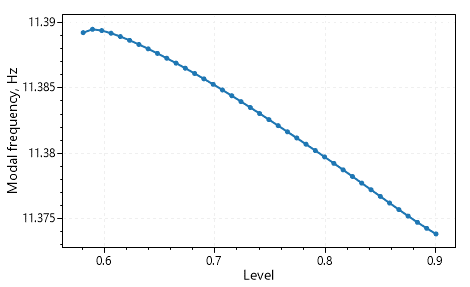
\includegraphics[width=0.65\linewidth]{natural-frequency}
	\caption{Собственная частота колебаний конструкции по тону АГИКр2, определенная по обобщенным характеристикам} \label{natural-frequency}
\end{figure}

\begin{figure}[H]
	\centering
	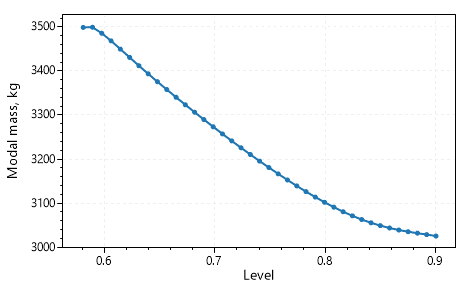
\includegraphics[width=0.65\linewidth]{general-mass}
	\caption{Обобщенная масса конструкции, соответствующая тону АГИКр2} \label{general-mass}
\end{figure}

\begin{figure}[!htb]
	\centering
	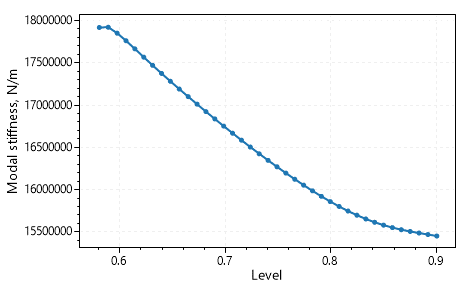
\includegraphics[width=0.65\linewidth]{general-stiffness}
	\caption{Обобщенная жесткость конструкции, соответствующая тону АГИКр2} \label{general-stiffness}
\end{figure}

\begin{figure}[!htb]
	\centering
	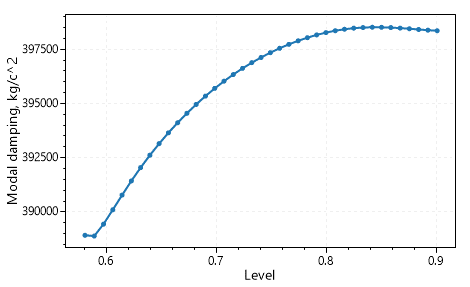
\includegraphics[width=0.65\linewidth]{general-damping}
	\caption{Обобщенное демпфирование конструкции, соответствующее тону АГИКр2} \label{general-damping}
\end{figure}

% -- Debug ------------------------------------------------------------------
%\end{document}